
\newcommand{\tg}[1]{%
  \tikz[baseline=0.06ex]\draw[fill=#1, draw=black, line width=0.75pt] (0,0) -- (0.2,0) -- (0.1,0.2) -- cycle;\xspace
}
\newcommand{\sq}[1]{%
  \tikz[baseline=0.06ex]\draw[fill=#1, draw=black, line width=0.75pt] (0,0) -- (0.2,0) -- (0.2,0.2) -- (0,0.2) -- cycle;\xspace
}
\newcommand{\tdA}{\tg{xblue}}
\newcommand{\tdB}{\tg{xcyan}}
\newcommand{\tdC}{\sq{xcyan}}
\newcommand{\tdD}{\sq{xlightcyan}}
\newcommand{\ellipseicon}[1]{%
  \tikz[baseline=-0.55ex]\shade[shading=radial, inner color=#1!100, outer color=#1!0, draw=none]
      (0,0) ellipse [x radius=0.35cm, y radius=0.15cm];\xspace
}

\begin{wrapfigure}{r}{0.45\textwidth}
    \centering
    \vskip -1.5\baselineskip
    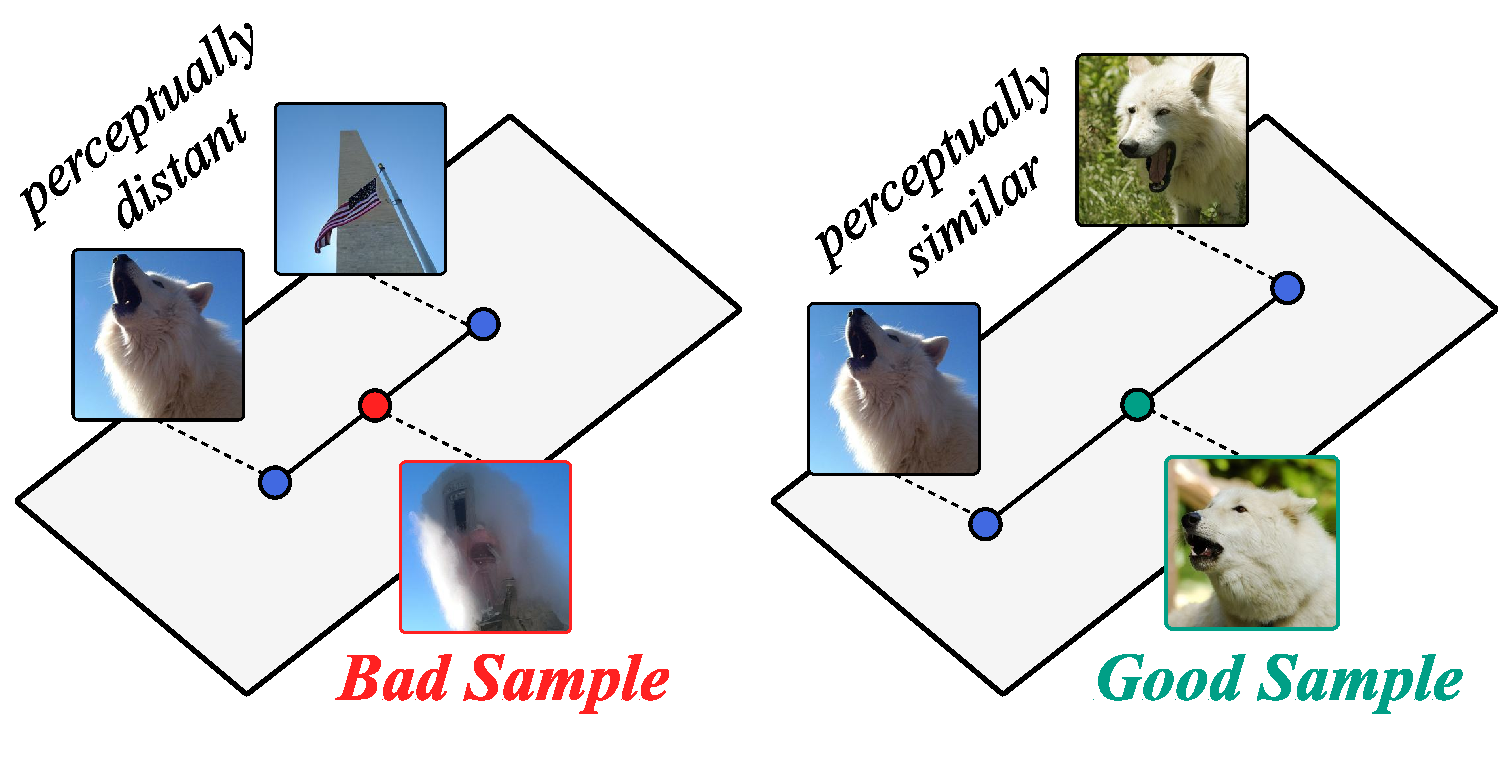
\includegraphics[width=0.45\textwidth]{figures/performance/good_generation}
    \vskip -\baselineskip
    \caption{\textbf{\xxgreen{Good} vs.\ \xred{bad} samples and their connection to \emph{perception}.}}
    \label{fig:good-generation}
    \vskip -2\baselineskip
\end{wrapfigure}